%Publication version
\documentclass[aps,twocolumn,prd,superscriptaddress,showpacs,nofootinbib,fixfloat]{revtex4}
%Draft version
%\documentclass[aps,prd,superscriptaddress,showpacs]{revtex4}
%\usepackage{doublespace}
\usepackage{graphicx}
\usepackage{dcolumn}
\usepackage{bm}
\usepackage{natbib}

%\topmargin+1cm

% Journals
\newcommand{\aaps}{{Astron.~Astrophys.~Supp.}}
\newcommand{\physrep}{{Physics~Reports}}
\newcommand{\araa}{{Annu.~Rev.~Astron.~Astrophys.}}
\newcommand{\aap}{{Astron.~Astrophys.}}
\newcommand{\apjl}{{Astrophys.~J.~Lett.}}
\newcommand{\apjs}{{Astrophys.~J.~Supp.}}
\newcommand{\aj}{{Astron.~J.}}
\newcommand{\mnras}{{Mon.~Not.~R.~Astron.~Soc.}}

% Making life easier
\newcommand{\be}{\begin{equation}}
\newcommand{\ee}{\end{equation}}
\newcommand{\bea}{\begin{eqnarray}}
\newcommand{\eea}{\end{eqnarray}}
\newcommand{\backten}{\!\!\!\!\!\!\!\!\!\!}

% useful symbols
\newcommand{\nhat}{\hat{\bf n}}
\newcommand{\kvec}{{\bf k}}
\newcommand{\edm}{\epsilon_{dm}}
\newcommand{\edmnow}{\epsilon_{dm,0}}
\newcommand{\sv}{\langle\sigma_Av\rangle}
\newcommand{\khat}{\hat{\bf k}}

% Fermi is usually italicized - use \Fermi\ for space after word
\newcommand{\Fermi}{{\slshape Fermi}}

% math functions, units
\newcommand{\Mpc}{{\rm ~Mpc}}
\newcommand{\sech}{{\rm ~sech~}}
\newcommand{\Tr}{{\rm ~Tr~}}
\newcommand{\threej}[6]{{\left( \begin{array}{ccc} #1 & #2 & #3 \\ #4 & 
   #5 & #6 \end{array} \right)}}

% Doug's units
\newcommand{\s}{{\rm ~s}}
\newcommand{\kms}{{\rm ~km/s}}
\newcommand{\g}{{\rm ~g}}
\newcommand{\cm}{{\rm ~cm}}
\newcommand{\km}{{\rm ~km}}
\newcommand{\mm}{{\rm ~mm}}
\newcommand{\mJy}{{\rm ~mJy}}
\newcommand{\Jy}{{\rm ~Jy}}
\newcommand{\MJy}{{\rm ~MJy}}
\newcommand{\MJypSr}{{\rm ~MJy~sr^{-1}}}
\newcommand{\JypSr}{{\rm ~Jy~sr^{-1}}}
\newcommand{\Hz}{{\rm ~Hz}}
\newcommand{\kHz}{{\rm ~kHz}}
\newcommand{\MHz}{{\rm ~MHz}}
\newcommand{\GHz}{{\rm ~GHz}}
\newcommand{\K}{{\rm ~K}}
\newcommand{\mK}{\rm ~mK}
\newcommand{\microK}{\mu{\rm K}}
\newcommand{\eV}{{\rm ~eV}}
\newcommand{\eVs}{{\rm ~eV/s}}
\newcommand{\keV}{{\rm ~keV}}
\newcommand{\MeV}{{\rm ~MeV}}
\newcommand{\GeV}{{\rm ~GeV}}
\newcommand{\TeV}{{\rm ~TeV}}
\newcommand{\pc}{{\rm ~pc}}
\newcommand{\kpc}{{\rm ~kpc}}
%\newcommand{\Mpc}{{\rm ~Mpc}}
\newcommand{\erg}{{\rm ~erg}}
\newcommand{\degree}{^{\rm o}}
\newcommand{\sigmav}{\langle\sigma_Av\rangle}
\def\la{\vcenter{\hbox{$<$}\offinterlineskip\hbox{$\sim$}}}
\def\ga{\vcenter{\hbox{$>$}\offinterlineskip\hbox{$\sim$}}}


% Necessary for appendices
\newcommand{\lmax}{{l_{\rm max}}}
\newcommand{\lmaxtwo}{{l_{\rm max}^2}}
\newcommand{\lmaxthree}{{l_{\rm max}^3}}


\newcommand\dpf[1]{{\bf (DPF: #1)}}

\begin{document}


\title{Is the 130 GeV Line Real? \\
  A Search for Systematics in the Fermi-LAT Earth Limb Data}

\author{Douglas P. Finkbeiner}
%\email{dfinkbeiner@cfa.harvard.edu}
\affiliation{Institute for Theory and Computation,
  Harvard-Smithsonian Center for Astrophysics, 
  60 Garden Street, MS-51, Cambridge, MA 02138 USA} 
\affiliation{Center for the Fundamental Laws of Nature,
  Physics Department, 
  Harvard University, 
  Cambridge, MA 02138 USA}

\author{Meng Su}
\affiliation{Institute for Theory and Computation,
  Harvard-Smithsonian Center for Astrophysics, 
  60 Garden Street, MS-51, Cambridge, MA 02138 USA} 

\author{Christoph Weniger}
\affiliation{Max-Planck-Institut f\"ur Physik, 
  F\"ohringer Ring 6, 
  80805 M\"unchen, Germany}

\begin{abstract} Our recent claims of a Galactic center feature in Fermi/LAT
  data at approximately 130 GeV have prompted an avalanche of papers proposing
  explanations ranging from dark matter annihilation to exotic pulsar winds.
  Because of the importance of such interpretations for physics and
  astrophysics, the threshold for discovery is unusually high.  This requires
  not only additional data, but a thorough investigation of possible LAT
  systematics.  While we do not have access to the details of each event
  reconstruction, we do have information about each event from the public
  event lists and spacecraft parameter files.  These data allow us to search
  for suspicious trends that could indicate a spurious signal.  In particular,
  the Earth limb photons provide a smooth reference spectrum for null tests.
  We examine these events and find a marginally significant 130 GeV feature in
  a small subset of the data.  This raises concerns about the 130 GeV Galactic
  center feature, even though we can think of no plausible model of
  instrumental behavior that connects the two.  A modest amount of additional
  limb data would tell us if the limb feature is a statistical fluke.  If the
  limb feature persists, it raises serious concerns about the Pass 7
  processing of $E > 100$ GeV events.
\end{abstract}

\pacs{}

\maketitle

\section{Introduction}
The search for dark matter takes many forms:  exploration of its astrophysical
properties, direct detection in underground labs, and even collider signatures
of WIMPs or related particles.  (cite reviews).   Etc. 

A gamma-ray line is a long-sought smoking gun for WIMP annihilation. 

We were not optimistic, because the branching ratio to lines is loop
suppressed, and one would have expected to see a continuum first in e.g. MSSM
models.  However, there are other models (e.g. MiDM) that allow high line to
continuum ratios.  In this work, we drop all theoretical prejudice and simply
ask if there is a line in the Galactic center spectrum. 

The first claim of a line around 130 GeV emerged from the work of Weniger
(cite), which grew out of an earlier search for other hard photon signals from
annihilations (Bringmann).  Weniger focused on spectral fitting to photon
events in regions of interest designed to maximize S/N.  He found a XXX sigma
signal at 130 GeV. 

Subsequent work by Su \& Finkbeiner approached the problem with template
fitting, assuming various profiles (Einasto, NFW, Gaussian) for the DM
distribution.  If the template is correct, this should allow extraction of the
DM signal with higher S/N.   This work found XXX sigma for an Einasto profile
centered $1.5\degree$ W of the Galactic center, and also suggest that there
may be two lines, at about 111 and 129 GeV.  The lower energy is tantalizing
because it matches the expected energy of a $Z\gamma$ line if the higher
energy is the $\gamma\gamma$ line. 

These papers have provoked theorists to try to reconcile the observations with
a number of theories (cite dozens of papers).  But all of this work depends on
the question:












10.  Direction of the orbital pole (upper panel) and Sun (lower panel)
for the events.   Note that some times of year these events do not
occur.





\begin{figure*}[p]
\centering
\includegraphics[width=0.6\textwidth]{plots/theta-E.ps}
\caption{Incidence angle $\theta$ vs. log $E$ for $Z > 105\degree$.  A blue
  box indicates the region $30\degree < \theta < 45\degree$ and 125 GeV $< E
  <$ 140 GeV, where an excess of events appear.  The vast majority of limb
  events are at $\theta > 60\degree$ because the telescope seldom points more
  than $50\degree$ from zenith, and the limb events are mostly at
  $Z>110\degree$.}
\label{fig:theta-E}
\end{figure*}


\begin{figure*}[p]
\centering
\includegraphics[width=0.6\textwidth]{plots/Ehist-all.ps}
\caption{Histogram of limb $(Z>105\degree)$ events vs. log($E$) for various
  ranges of $\theta$. The position of the 130 GeV line is indicated (red
  dotted line).  Note the excess in the $30\degree < \theta < 45\degree$ bin,
  which contains about 5\% of the limb events.}
\label{fig:Ehist-all}
\end{figure*}

\begin{figure*}[p]
\centering
\includegraphics[width=0.6\textwidth]{plots/theta-phi.ps}
\caption{Line events (125 GeV $< E <$ 140 GeV) in physical detector angle
  coordinates ($\theta, \phi$).  The $30\degree < \theta < 45\degree$ events
  are blue in this and following panels.  }
\label{fig:theta-phi}
\end{figure*}

\begin{figure*}[p]
\centering
\includegraphics[width=0.6\textwidth]{plots/l-b.ps}
\caption{Same events, projected as an equal-area plot of Galactic $(\ell, \sin
  b)$.  The majority of high-incidence limb events appear near the orbital
  pole, which precesses around the celestial pole.  This pattern is expected
  from the observing strategy. }
\label{fig:l-b}
\end{figure*}




\begin{figure*}[p]
\centering
\includegraphics[width=0.6\textwidth]{plots/rockangle.ps}
\caption{Rock angle -- need to add red and blue to this plot...
}
\label{fig:rock}
\end{figure*}

\clearpage
Now for some text...


Possible systematic errors:

- Extra events

{\bf Low energy photons:} Events would have to be mistakenly mapped from
either lower energy ($E \la 10$ GeV) gammas or much lower energy photons
(X-rays from the 1E $1740.7-2942$ microquasar?  511 keV photons?) in which the
Galactic center is much brighter.  It is difficult to see how this could
happen.

{\bf High energy photons:} At $E > 100$ GeV, the Galactic center is only
modestly brighter than the surrounding regions, so there are not enough
photons available.

{\bf Particle contamination:} If monochromatic photons from the limb are
difficult to explain, it is even harder to understand how mono-energetic
particles could be present. 

{\bf Effective area error:} An error in the LAT effective area (e.g. various
cuts are less restrictive for some reason) for $30\degree < \theta <
45\degree$ could explain the limb photons, but would also produce a line
everywhere in the Galactic plane.  No such line is seen outside of the GC. 

From these considerations, we conclude that there is no way for the limb line
to be caused by extra events. 

However, it is still plausible that there is a more subtle energy mapping
error that distorts the energy scale near 130 GeV.  In the next section, we
argue that this is a reasonable explanation of the limb line, but not of the
GC lines. 

\section{Observation of the Galactic Center}
Figure \ref{fig:l_phi} and \ref{fig:l_theta} show the distribution of event
incident angles as function of the Galactic longitude. From
Fig.~\ref{fig:l_phi} it is apparent that the Galactic center is predominantly
observed under $\phi\approx 0^\circ$ and $\phi\approx 180^\circ$. This is
because the path of the Sun over the sky actually intersects with the Galactic
center, and Fermi keeps the solar panels aligned to the Sun. This anual
modulation is clearly visible in Fig.~\ref{fig:time_phi}. To check whether
this behaviour could cause the 130 GeV feature, we plot in
Fig.~\ref{fig:spectrum_phi} the energy distribution of events with impact
angles close to $\phi\approx0^\circ$ and $\phi\approx180^\circ$. No line at
130 GeV appears.

\begin{figure*}
\centering
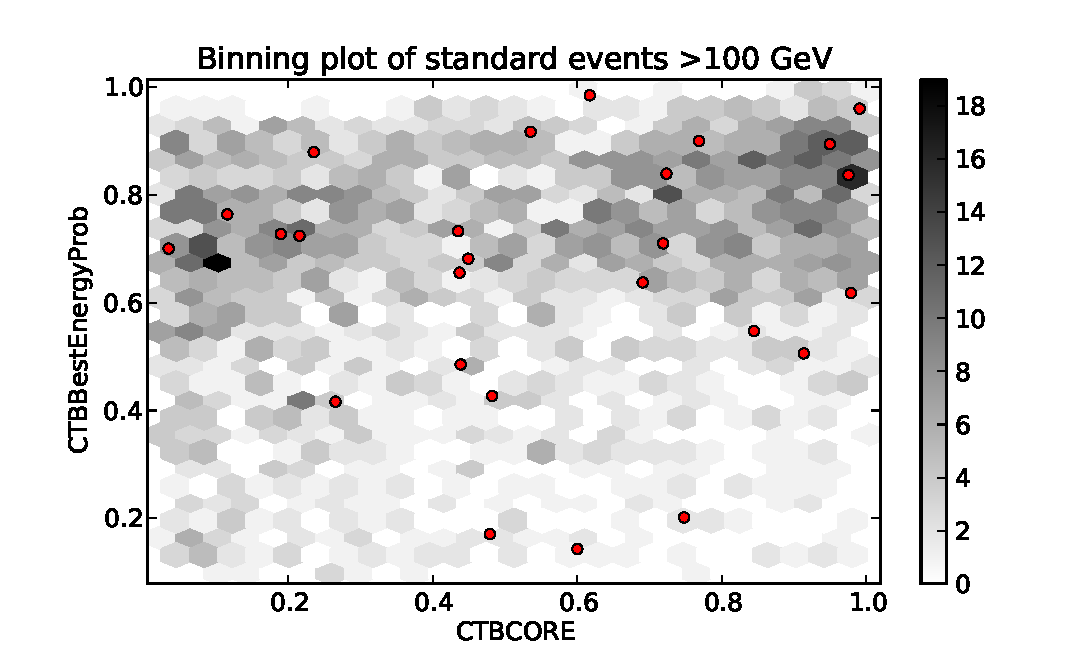
\includegraphics[width=0.6\textwidth]{plots/CTBCORE_CTBBestEnergyProb.eps}
\caption{Distribution of CTBCORE (the probability that the direction estimate
is good) and CTBBestEnergyProb (the probability that the best energy chosen
from the two energy estimators is correct) for GC events (in red), compared to
average distribution for $>50$ GeV events.}
\label{fig:CTBquality}
\end{figure*}

\begin{figure*}
\centering
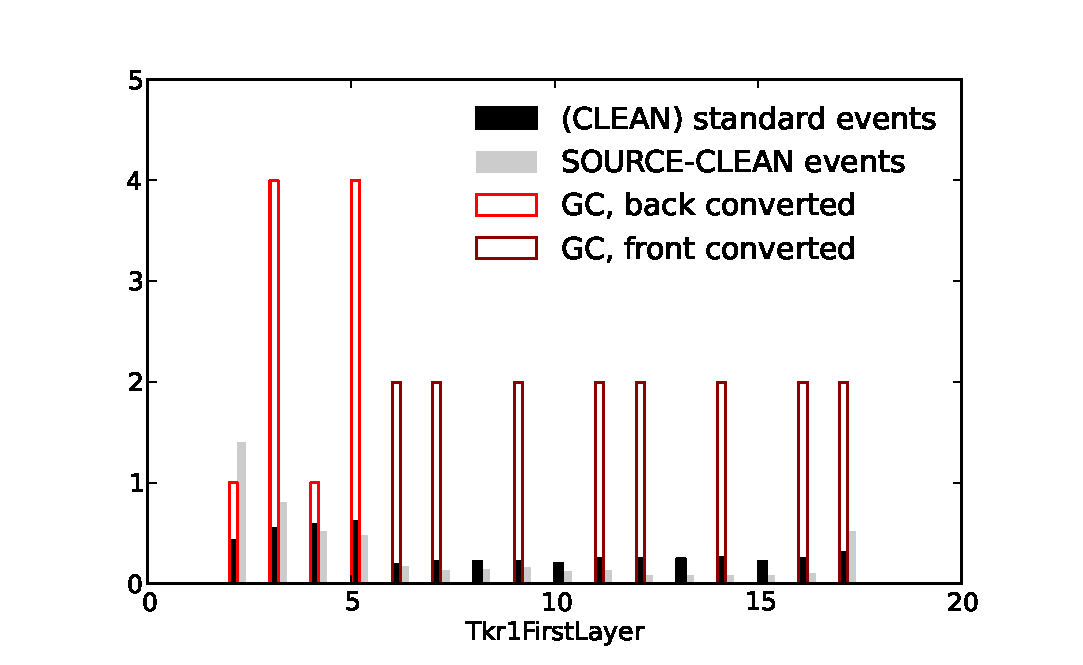
\includegraphics[width=0.6\textwidth]{plots/Tkr1FirstLayer.eps}
\caption{First tracker layer to show evidence of a particle hit for the best
track reconstruction. Tracker layers are 0-17 where 0 is closest to the
calorimeter, and 6-17 (2-5) corresponds to front- (back-)converting events
(tracker layers 0 and 1 come without conversion foils). The gray bars show the
distribution averaged over all $>100$ GeV events, the green/red bars show the
distribution for the GC line.}
\label{fig:Tkr1FirstLayer}
\end{figure*}

\begin{figure*}
\centering
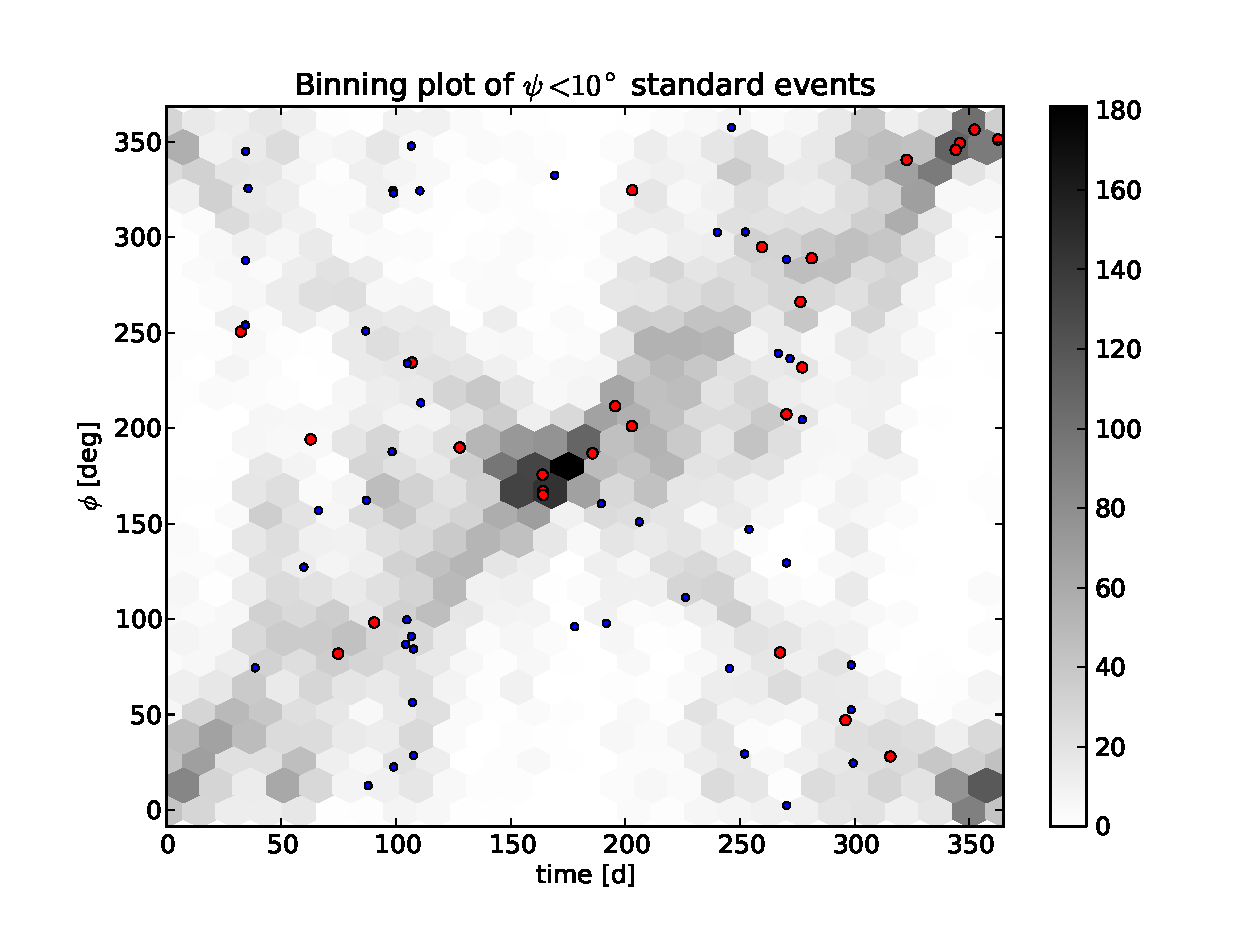
\includegraphics[width=0.6\textwidth]{plots/TIME_PHI.eps}
\caption{PHI distribution of GC events as function of time modulo one year
(with Jan 1st as origin). In Dec (Jun) the sun stands in Sagittarius (anti
galactic center). In these periods, most events are observed under
$\phi\approx 0^\circ$ ($\phi\approx 180^\circ$), since the instrumental x-z
plane is fixed by the sun to keep the solar panels aligned.}
\label{fig:time_phi}
\end{figure*}

\begin{figure*}
\centering
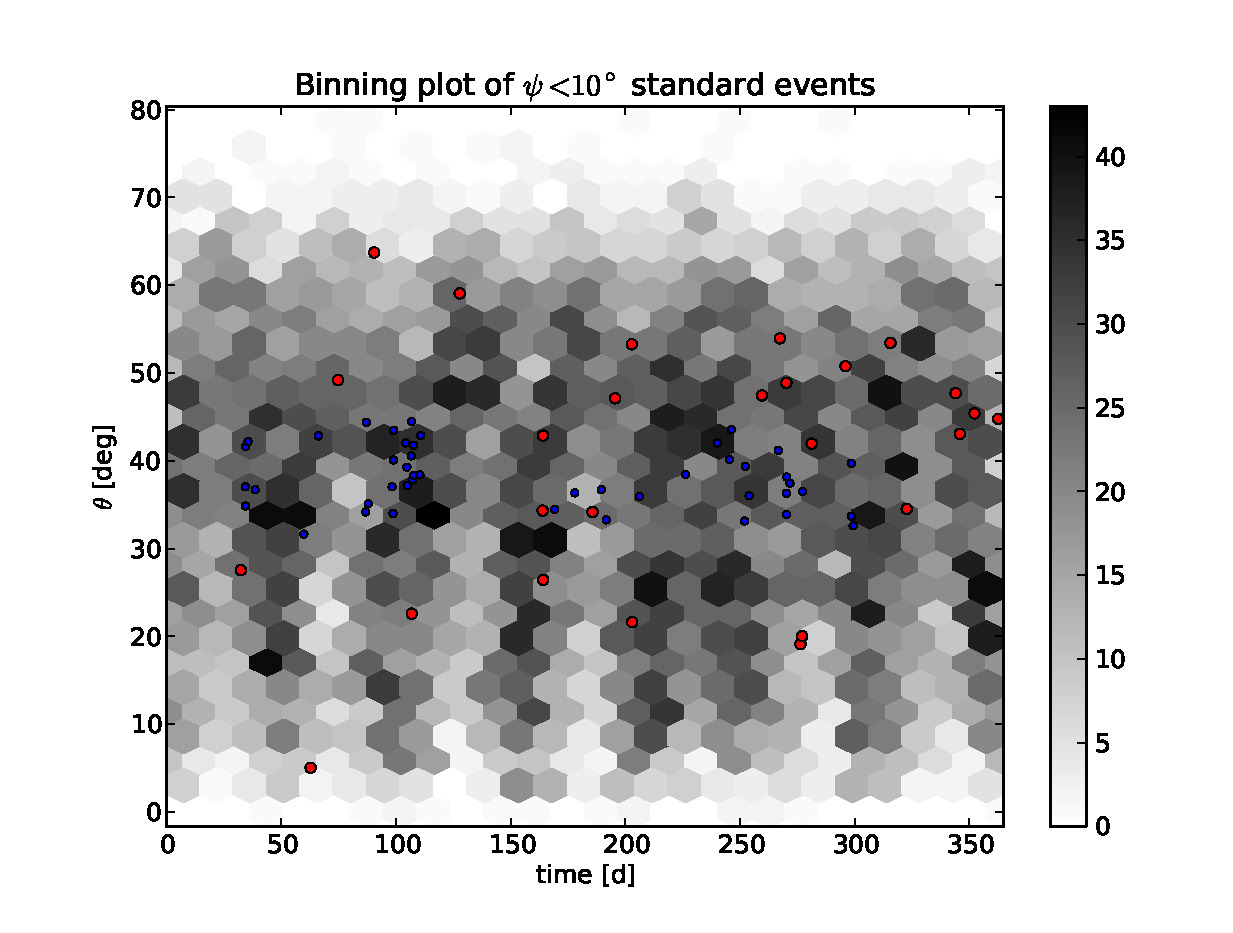
\includegraphics[width=0.6\textwidth]{plots/TIME_THETA.eps}
\caption{Same as Fig.~\ref{fig:time_phi}, but for THETA.}
\label{fig:time_theta}
\end{figure*}

\begin{figure*}
\centering
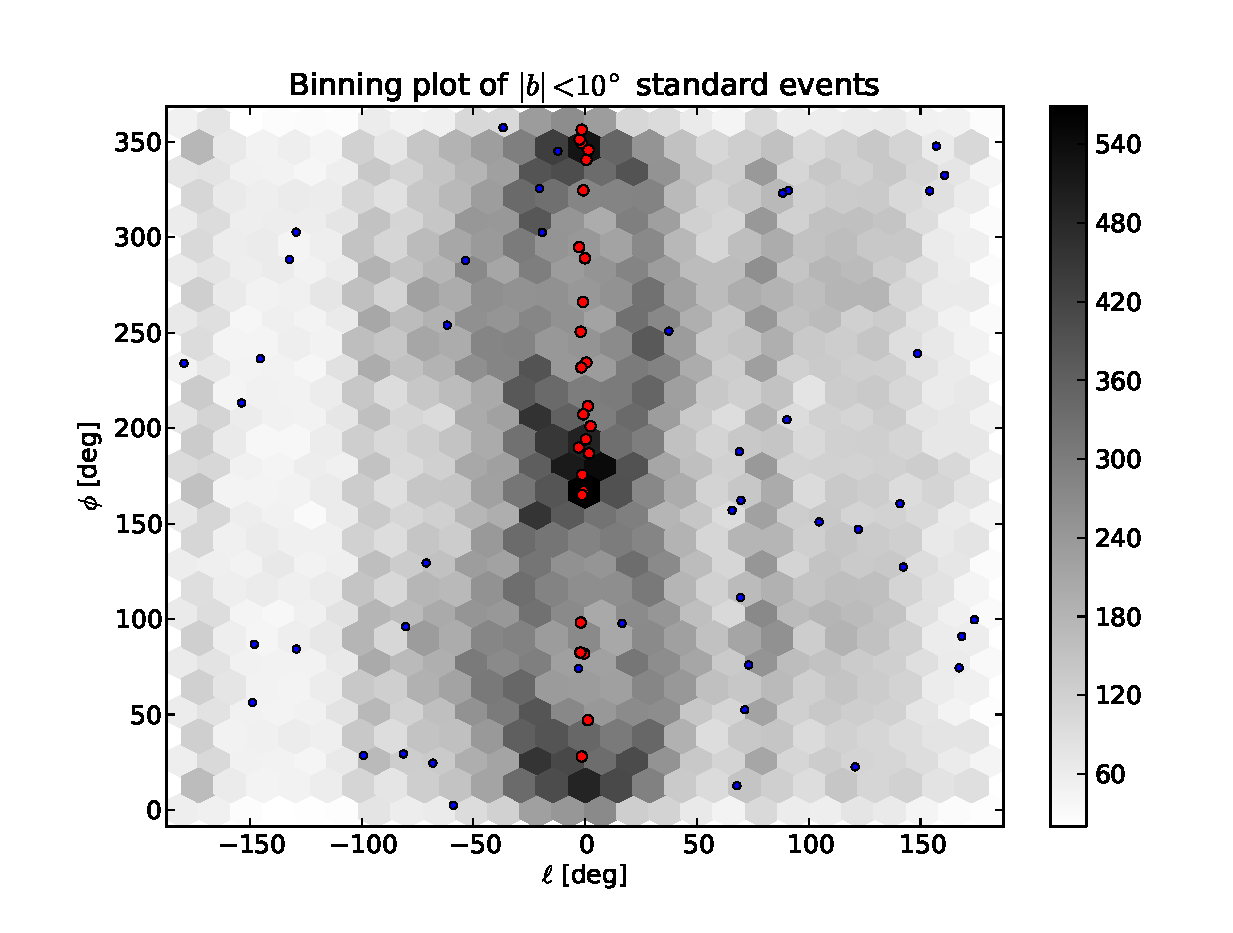
\includegraphics[width=0.6\textwidth]{plots/L_PHI.eps}
\caption{PHI distribution of events along the galactic disk. Close to the GC, the
distribution becomes significantly biased.}
\label{fig:l_phi}
\end{figure*}

\begin{figure*}
\centering
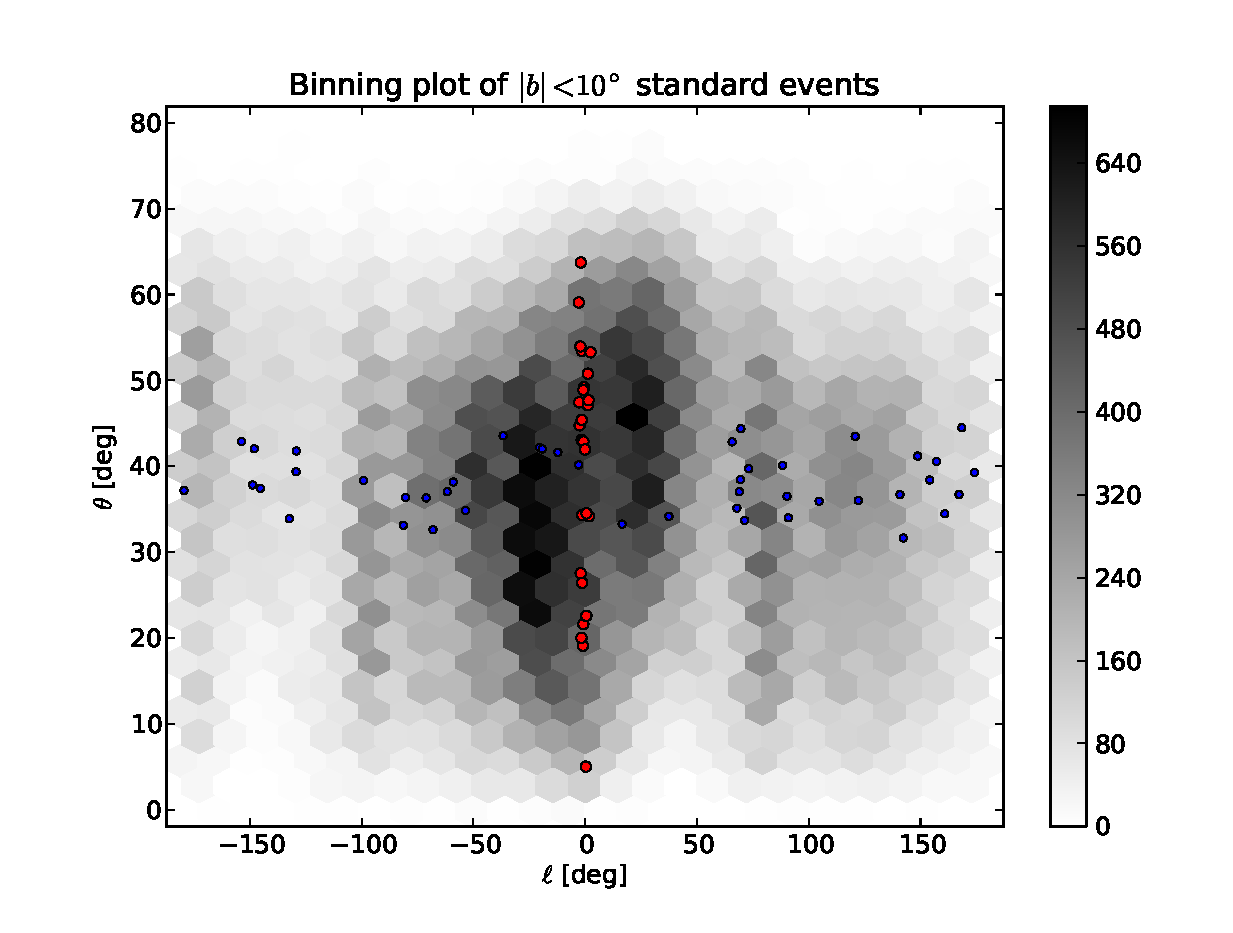
\includegraphics[width=0.6\textwidth]{plots/L_THETA.eps}
\caption{Same as Fig.~\ref{fig:l_phi}, but for THETA.}
\label{fig:l_theta}
\end{figure*}

\begin{figure*}
\centering
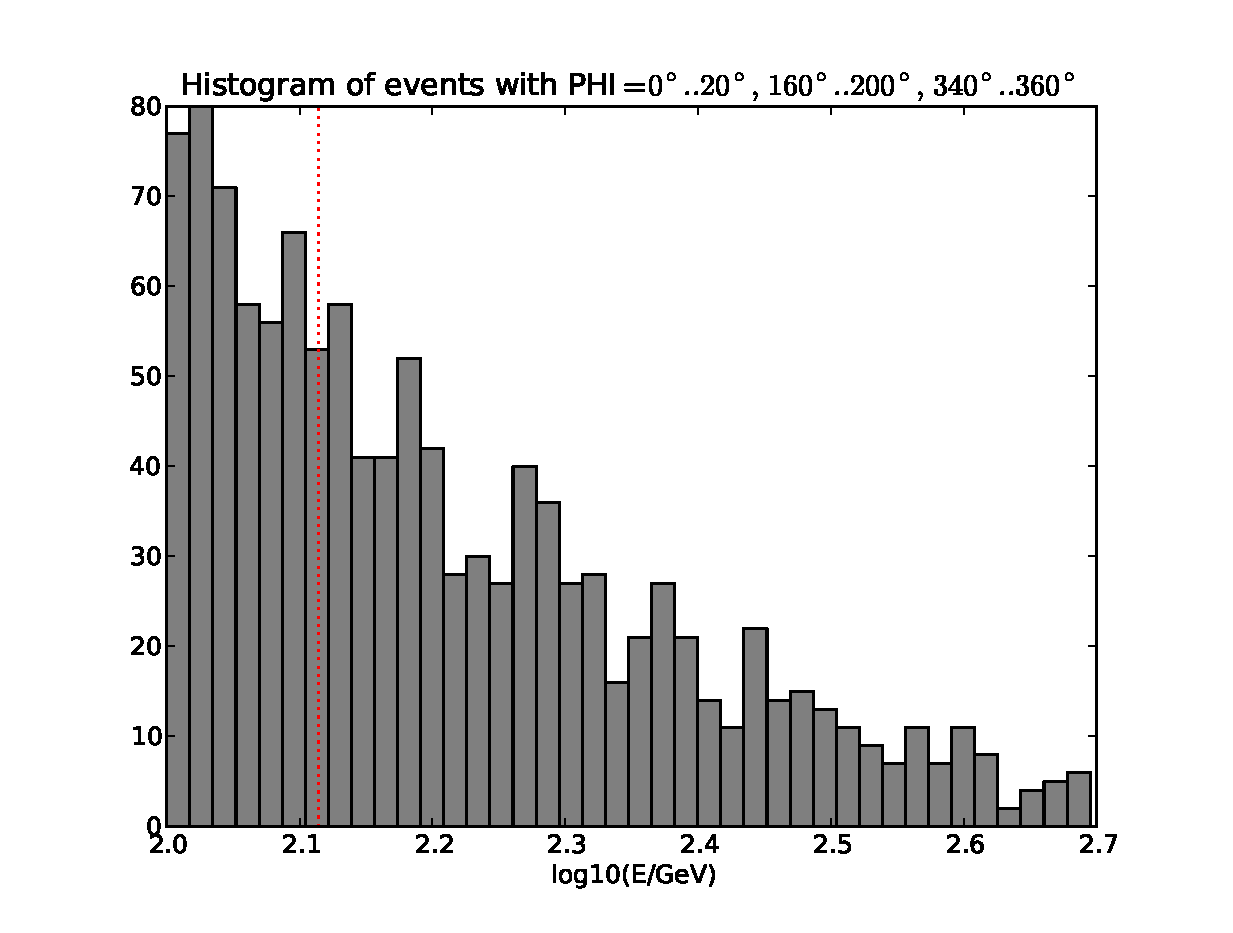
\includegraphics[width=0.6\textwidth]{plots/spectrum_phi.eps}
\caption{Energy distribution of all-sky events with incident angles close to
the x-z plane (perpendicular to the solar panels). The red dotted line
indicates 130 GeV.}
\label{fig:spectrum_phi}
\end{figure*}

\begin{figure*}
\centering
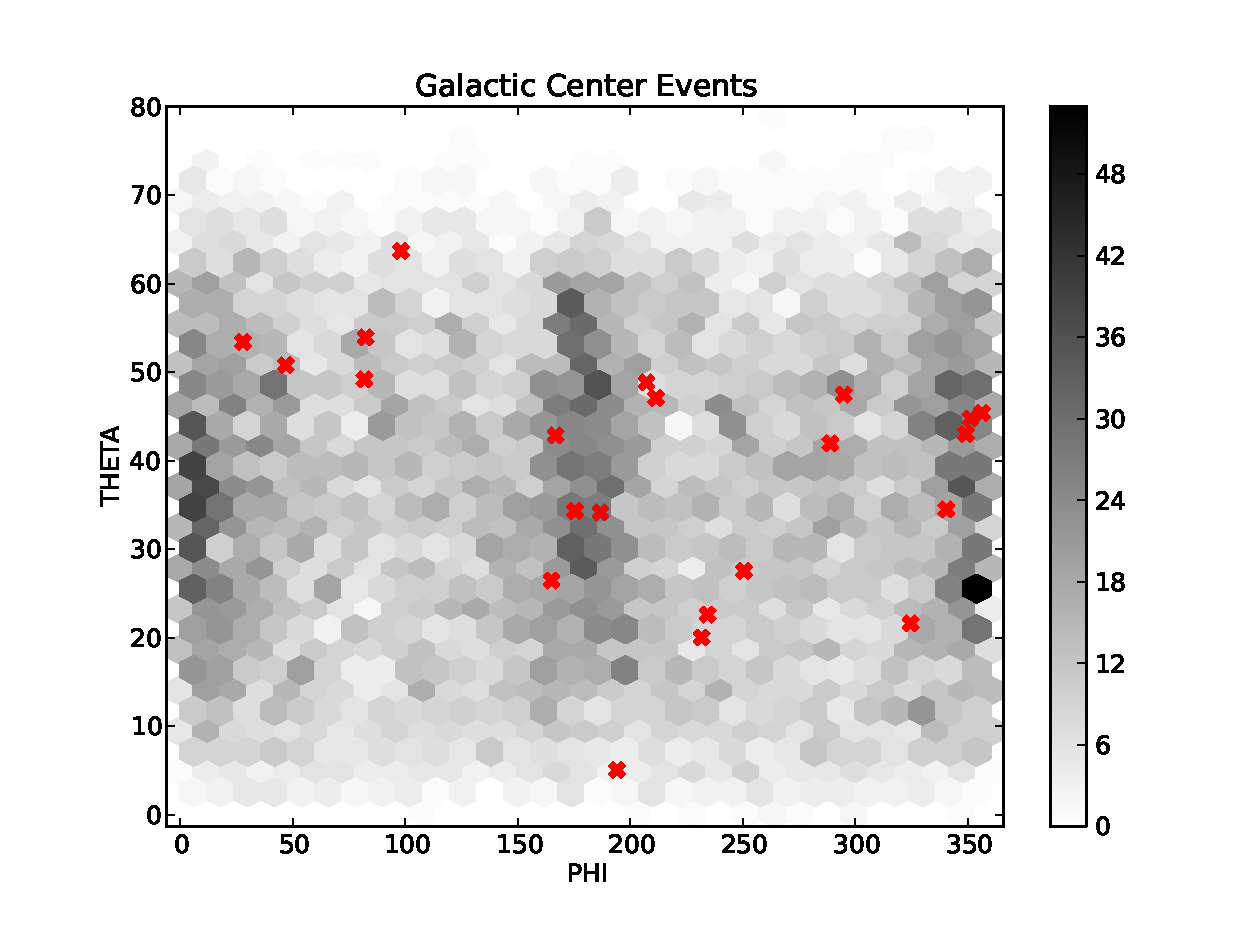
\includegraphics[width=0.6\textwidth]{plots/GC_THETA_PHI.eps}
\caption{THETA and PHI distribution of GC line (red crosses), compared to
distribution of all $>10$ GeV events within $10^\circ$ of the GC.}
\label{fig:gc_theta_phi}
\end{figure*}


\section{Energy mapping error: a model for the limb bump}
Given the difficulty in explaining the excess any other way, we consider the
possibility that the limb bump results from an energy mapping error.  We
propose a simple model, in which the mapping from true energy to reported
energy, $E(E_t)$, is linear except for a bump near some reference energy.
Smooth low-level perturbations over large energy scales are not relevant here,
and could be absorbed in the effective area calibration.  In order to include
a small-scale bump in the response, we introduce a local compact perturbation
in the form of a Gaussian.  It is convenient to work in logarithmic
quantities, so we take $x=\log E_t, y=\log E$, and
\be
\label{eq:yofx}
y=x - A\sigma \exp\left(\frac{1}{2}-\frac{(x-x_0)^2}{2\sigma^2}\right),
\ee
where $A$ is a dimensionless amplitude of the bump ($-1<A<1$ is required
for monotonicity of $y(x)$), $x_0$ is a reference energy, and $\sigma$ is the
width of the bump (see Figure \ref{fig:bumpmodel}).
The effect of the distortion is to change the true spectrum $dN/dx =
dN/dlog(E_t)$ into an observed spectrum
\be
\label{eq:dndy}
\frac{dN}{dy} = \frac{dN}{dx} \left(\frac{dy}{dx}\right)^{-1} ,
\ee
with
\be
\label{eq:dydx}
\frac{dy}{dx} = 1 + A\sigma \exp\left(\frac{1}{2}-\frac{(x-x_0)^2}{2\sigma^2}\right)
\frac{x-x_0}{\sigma^2}.
\ee
Note that that the extreme values of $dy/dx = 1 \pm A$ occur at $x-x_0 = \pm
\sigma$ and at $y=x_0(\pm1-A)\sigma$.  Assuming the true limb spectrum is a
power law, we may apply this factor to obtain a model spectrum, and maximize
the Poisson likelihood of observing the data given the model.

To illustrate that this model can generate a spectrum similar to the limb bump
spectrum, we show 10 random realizations of a $dN/dE \sim E^{-2.6}$ spectrum
with this distortion in Figure \ref{fig:bumpmodelmany}.
Some of these look very similar to the bump in Figure \ref{fig:Ehist-all}.


\section{Future}
Ways to progress.

One to two weeks of additional limb data would provide an exposure comparable
to teh limb photons used here.  One option would be to release comissioning
data from early in the survey, if they are thought to be of sufficient
quality.  Otherwise, new limb observations could be undertaken, in order to
test teh reality of the 130 GeV limb feature.  

If the 130 GeV feature is not replicated, it can be dismissed as a statistical
fluke.  If it reappears, a deppr inestigation into its cause is warrented.  

even then, it is a challenge to understand how such an instrumental feature
could be mapped so precisely onto a localized region within 5-10 degrees of
the GC.  The GC is not near the path of the orbital pole, nor its axis of
precession.  The orbital phase, precession, Earth's orbit, and time of year
are all well mixed by the few $\times10^4$ orbits and 25 precession cycles
over 1500 days.  We have shown that the events in question are drawn from
every part of event and spacecraft parameter space available in teh public
files.  In the absence of any model of instrumental behavior that explains how
these events land near the GC and not elsewhere in the Galactic plane, it is
far fetched to say that they invalidate a result with a local signiifcance of
$p\approx10^{-9}$.  



\begin{figure*}[p]
\centering
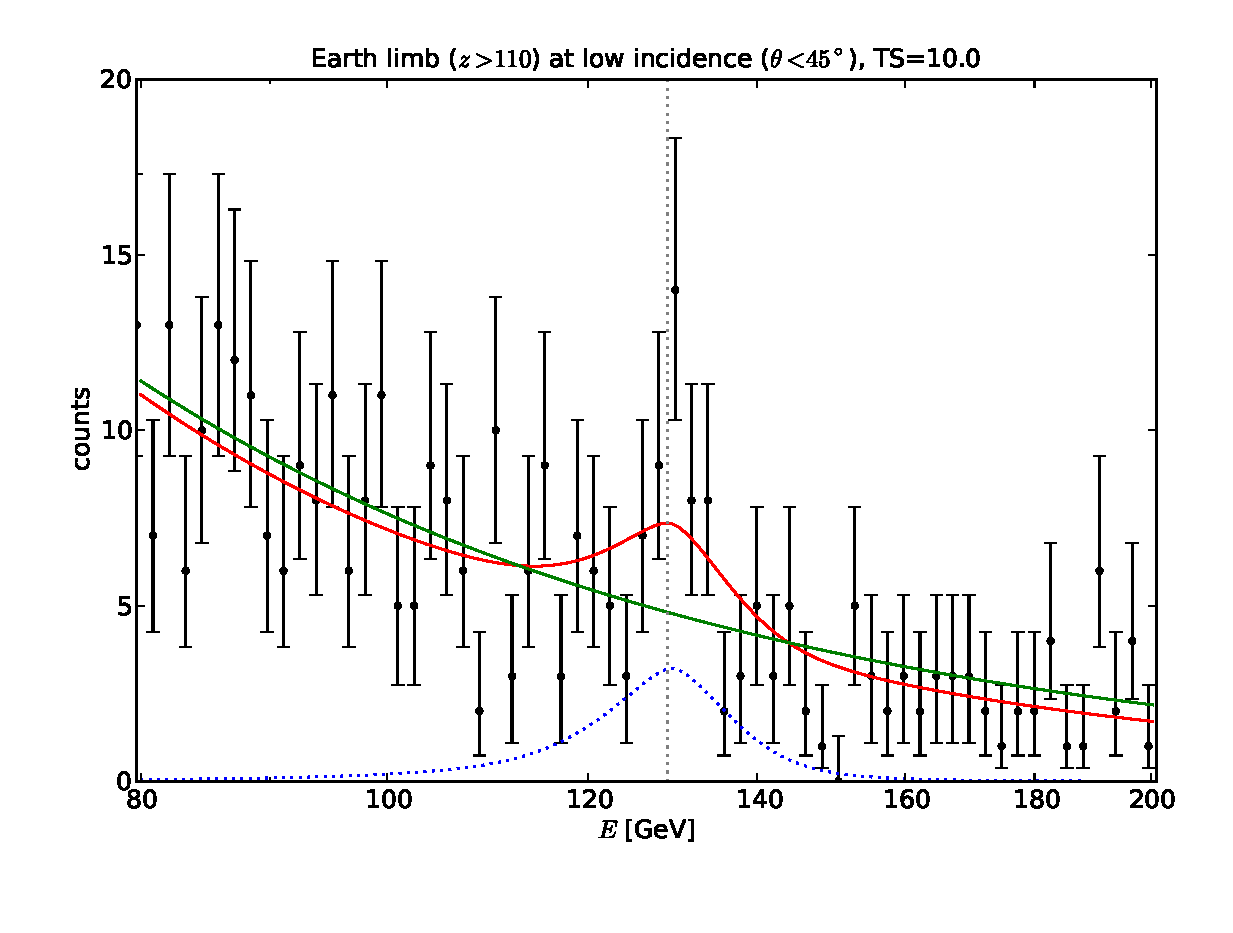
\includegraphics[width=0.6\textwidth]{plots/albedo_line_thetaCut.eps}
\caption{Fit of a monochromatic line at 129 GeV to the low impact angle Earth
  limb data. A 129 GeV line has a local significance of 3.2$\sigma$.
}
\label{fig:albedoline}
\end{figure*}

\begin{figure*}[p]
\centering
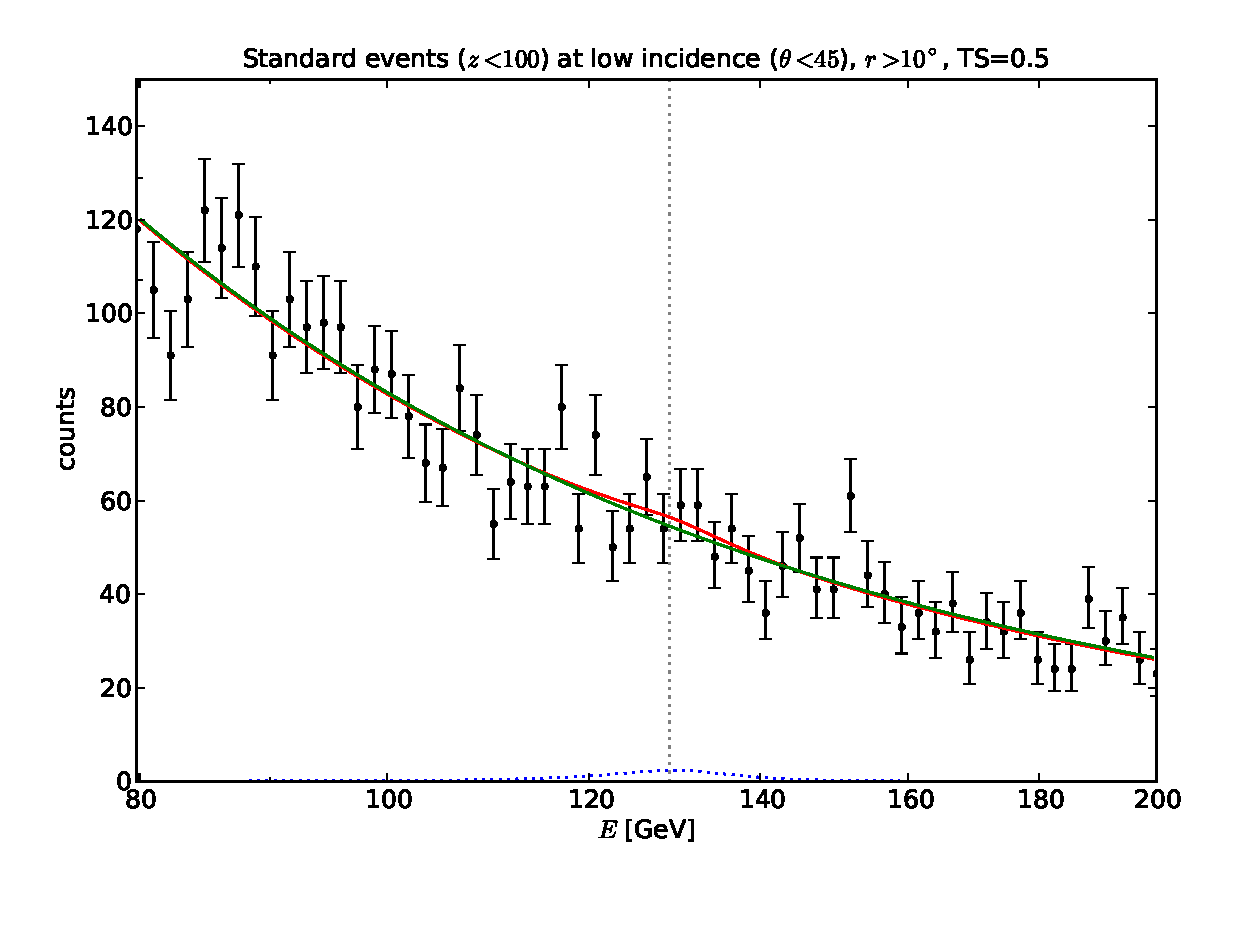
\includegraphics[width=0.6\textwidth]{plots/noalbedo_line_thetaCut.eps}
\caption{Same as Figure \ref{fig:albedoline}, but for the low
impact angle standard events. The inner $10^\circ$ around the Galactic center
is masked out. We find no indication for a line at 129 GeV.
}
\label{fig:noalbedoline}
\end{figure*}

\begin{figure*}[p]
\centering
\includegraphics[width=0.6\textwidth]{plots/theta-time.ps}
\caption{Distribution of impact angles $\theta$ as function of
time. Red (black) dots show the events from the Galactic center (Earth limb)
130 GeV feature; yellow(gray) dots show all standard (Earth limb) events for
comparison.
}
\label{fig:cw3}
\end{figure*}

\begin{figure*}[p]
\centering
\includegraphics[width=0.6\textwidth]{plots/theta-time-rock52.ps}
\caption{Same as [theta-time.png], but with rocking angles above
$52^\circ$ excluded.
}
\label{fig:cw4}
\end{figure*}

\begin{figure*}[p]
\centering
\includegraphics[width=0.6\textwidth]{plots/limb_bump_model.ps}
\caption{Upper panel: function mapping true energy $E_t$ to reported energy
  $E$ (see Eqs. \ref{eq:yofx} and \ref{eq:dydx}).  Middle panel: The effect of
  this mapping on a spectrum of constant $dN/d\log E_t$, as in Eq.
  \ref{eq:dndy} (red line) and also for mock data (black histogram).  Lower
  panel: Same, but for $dN/dE \sim E^{-2.6}$.  }
\label{fig:bumpmodel}
\end{figure*}

\begin{figure*}[p]
\centering
\includegraphics[width=0.6\textwidth]{plots/limb_bump_model_many.ps}
\caption{Ten mock spectra of an underlying spectrum $dN/dE \sim E^{-2.6}$,
  distorted according to Eq. \ref{eq:dndy}.  Note the similarity to the
  $30\degree < \theta < 45\degree$ panel in Figure \ref{fig:Ehist-all}.  
}
\label{fig:bumpmodelmany}
\end{figure*}

\begin{figure*}[p]
\centering
\includegraphics[width=0.6\textwidth]{plots/limbfits.ps}
\caption{Fits of the energy mapping model to limb data for various ranges of
  inclination angle $\theta$.  The vertical dotted line corresponds to 130
  GeV.  The test statistic ($2\Delta\ln L$) for the best fit model (green
  line) relative to the null hypothesis (red line) is given, along with the
  significance, expressed in ``sigma'' including a penalty for the 3
  additional degrees of freedom.  The deviation from linearity is only
  significant in the $30\degree < \theta < 45\degree$ panel.}
\label{fig:limbfits}
\end{figure*}




\section{Conclusions}

\clearpage
\appendix
\section{This here is an appendix}

Here are a bunch of plots that are good to have, and could have shown
something interesting, but do not. 

\begin{figure*}[p]
\centering
\includegraphics[width=0.45\textwidth]{plots/timehist.ps}
\caption{Time histogram (1-day bins) of suspicious limb events and all limb
events.  The suspicious events are only observed at high rocking
angles that occur during pointed observations.
}
\label{fig:timehist}
\end{figure*}


\begin{figure*}[p]
\centering
\includegraphics[width=0.45\textwidth]{plots/Ehist-frontback.ps}
\caption{Energy histogram as in Figure \ref{fig:Ehist-all}, but for front
  (upper panel) and back (lower panel) converting events.  The 130 GeV excess
  appears equally in front and back converting events. 
}
\label{fig:Ehist-frontback}
\end{figure*}



\begin{figure*}[p]
\centering
\includegraphics[width=0.45\textwidth]{plots/theta-E-frontback.ps}
\caption{Same as ??? but for front and back converting events.}
\label{fig:theta-E-frontback}
\end{figure*}

\begin{figure*}[p]
\centering
\includegraphics[width=0.45\textwidth]{plots/geo-lonlat.ps}
\caption{Distribution of suspicious events in Earth longitude and latitude
(upper panel) and satellite zenith RA,dec (lower panel).   The
avoidance of the SAA leaves a hole in the upper panel.}
\label{fig:geo-lonlat}
\end{figure*}

\begin{figure*}[p]
\centering
\includegraphics[width=0.45\textwidth]{plots/spacecraft-zx.ps}
\caption{Direction of spacecraft Z axis (boresight direction) and X axis
(Solar panel direction) for the suspicious events.
}
\label{fig:spacecraft-zx}
\end{figure*}

\begin{figure*}[p]
\centering
\includegraphics[width=0.45\textwidth]{plots/earth-az.ps}
\caption{Zenith angle vs. Earth azimuth angle for limb photons.  As expected,
  the $\theta > 60\degree$ limb photons observed in survey mode are seen
  predominantly to the north and south azimuth directions, i.e approximately
  perpendicular to the orbit direction.  }
\label{fig:earth-az}
\end{figure*}

\begin{figure*}[p]
\centering
\includegraphics[width=0.45\textwidth]{plots/sun.ps}
\caption{Blue, red, and black events as a function of orbital precession phase
  (upper panel) and time of year (lower panel).  Note that there are only
  about 6 months of the year during which the 38 limb events are seen. 
}
\label{fig:sun}
\end{figure*}


\bibliography{systematics}

\end{document}
